% Metódy inžinierskej práce

\documentclass[11pt,slovak,a4paper]{article}

\usepackage[slovak]{babel}
%\usepackage[T1]{fontenc}
\usepackage[IL2]{fontenc} % lepšia sadzba písmena Ľ než v T1
\usepackage[utf8]{inputenc}
\usepackage{graphicx}
\usepackage{url} % príkaz \url na formátovanie URL
\usepackage{hyperref} % odkazy v texte budú aktívne (pri niektorých triedach dokumentov spôsobuje posun textu)
\usepackage{pdfpages}
\usepackage{cite}
\usepackage{dirtytalk}
\usepackage{indentfirst}
%\usepackage{times}

\graphicspath{ {./graphics/} }

\pagestyle{headings}

\title{Nový spôsob vzdelávania pomocou fenoménov\thanks{Semestrálny projekt v predmete Metódy inžinierskej práce, ak. rok 2020/21, vedenie: Mgr. Martin Sabo, PhD.}} % meno a priezvisko vyučujúceho na cvičeniach

\author{Rastislav Brna\\[2pt]
	{\small Slovenská technická univerzita v Bratislave}\\
	{\small Fakulta informatiky a informačných technológií}\\
	{\small \texttt{xbrna@stuba.sk}}
	}

\date{\small 10. december 2020}



\begin{document}

\maketitle

\begin{abstract}
	Vzdelávanie pomocou fenoménov je vzdelávanie v ktorom neexistujú 
	tradičné predmety ale vzdeláva sa na základe väčších tém ktoré sa rozoberajú zo všetkých strán.
	Jednu tému vieme rozobrať z fizikálneho, geografického, matematického, dejepisného alebo iného 
	hladiska. Tento štýl vzdelávania by mal zlepšit pochopenie učiva, keďze ludzký mozog vie spájať 
	si súvislosti medzi vecami omnoho lepšie ako si pamätať fakty naspamäť. V niektorých krajinách ktoré
	patria medzi lídrov vo vzdelávaní sa takýto systém už pomaly začína používať v praxi. Štúdia z turecka,
	potvrdila zlepšenie priemeru študentov o viac ako 10\%. Taktiež tento typ vzdelávania pomohol študentom 
	si dlhšie zachovať znalosťi ktoré nadobudly.\cite{jcer} 
\end{abstract}

\section{Úvod}

Svet a technológie idú dopredu ale sposob vzdelávanie je zastaralý a stovky rokov rovnaký. Znalosti potrebné k
životu sa menia a preto sa potrebuje prispôsobiť aj vzdelávanie. Aktuálny vzdelávací systém vo väčšine krajín 
rozdeluje vzdelávanie na určité smery(predmety), núti študentov sa učit vaľa veci z pamäti, vyvíja zbytočný tlak
a nezmyselne stresuje študentov už od útleho veku. Vzdelávanie na základe
fenoménov (Phenomenon-Based Learning) je metódou vzdelávania ktorá by mala zvýšit efektivitu vzdelávania
a dodať študentom lepšiu zručnosť, kreativitu, kritické myslenie, a schopnosť koloaborovať. Závisí na študovaní
fenoménu reálneho sveta z rôznych smerov pomocou čoho prepája hranice medzi školskými predmetami ako ich poznáme.
Mení vysvetlovanie novej látky z vysvetlenia učiva, vhoršom prípade len napísania poznámok z látky na tabulu na úvádzanie
študentov do témy cez zauhjímavé príbehy alebo hry a nabádanie ich k otázkam vďaka ktorým si znalosť témy osvoja a hlbšie zapametajú.
Aktívne núti študentov kolaborovať medzi sebov a zúčastnovať sa na spoločných aktivitách za účelom riešenia
problémov a odpovedania na otázky. 
\cite{pblf}

\section{Využitie modrných technológií}

Vzdelávanie pomocou fenoménov zahŕňa moderné technológie ale pri použitý správnych edtech (vzdelávacie technológie) nástrojov v správny čas.
Keďže nieje možné najnovšie informácie vyučovať z tradičných učebníc, čo môže spôsobiť ich zánik, tak sa vyučuje pomocou informácií z internetu, najme z
Otvorených vzdelávacých zdrojov (OERs). Študenti už nemusia závisieť od toho, čo učebnica ponúka. Namiesto toho môžu študenti zhromažďovať informácie z veľkého množstva zdrojov.
Študenti majú tak prístup k informáciám prostredníctvom digitálnych medií, ako sú videá, hry, vedecké štúdie a dalšie dokumenty. Učiteľom sa zdá OER prospešné kvôli výraznej úspore času a umožnuje aj jednoduchšie plánovanie.
\cite{fsew}

\subsection{Virtuálna realita}

Okrem bežných technológii sa tiež začína používať aj jedna z najmodernejších technológií a to virtuálna a rozšírená realita. Pri kombinácií so vzdelávaním pomocou fenoménov
to vytvára ešte väčší záujem študentov. Jedna vec je síce vidieť kresbu, fotografiu, 3D model alebo dokonca video. Avšak s využitím rozšírenej alevbo virtuálnej reality 
sa prekonávajú hranice pasívnej konzumácie obsahu a prichádza k plnému zapojeniu študanta do interaktívneho sveta. Virtuálne učebne a simulácie môžu študentom poskytnúť rýchle, efektívne a pútavé zážitky.
\cite{pbldc}
 
\subsection{Online}

Veľa možností ktoré vzdelávanie pomocou fenoménov ponúka, pri online výučbe zanikajú. Online výučba je viac orientovaná na obsah ako priamu fyzicku interakciu. Čo z jednej strany uberá na kvalite ale taktiež otvára nové možnosti
ako zapojiť viac médií. Taktiež to požaduje od študentov aby väčšiu samostatnosť pri štúdiu, avšak základ tohoto typu vzdelávania je zachovaný len nieje možné študentom poskytnúť všetky výhody ako je prima interakcia, technológie ako
virtuálna a rozšírená realita a kolaborácia. Kontakt medzi žiakmi a učitelom alebo medzi žiakmi samotnými môže byť pri dobrom pripojení zachovaný.
\cite{outdacc}
Z pohladu žiakov nieje online výučba lepšia ako klasická ale napríklad štúda \cite{ELZAINY} z univerzity Qassim v Buraidahu v Saudskej arábii zistila že viac ako 58\% študentov je veľmi spokojních s online vzdelávaním.


\section{Výsledky štúdii}

\subsection{Turecko}

Štúdia z turecka \cite{jcer} skúmala vzdelávanie na základe fenoménov pre vyučovanie Informačných a komunikačných technológií
kôli chýbajúcemu praktickému využitiu tohoto predmetu. Na troch rôznych základných školách vybrali zo siedmej, ôsmej a deviatej
triedy spolu 121 študentov. V ôsmej triede bolo iba okolo 8 študentov, takže jej výsledok môže byť ovplyvnený lepším pomerom študentov
k učitelom. Študentov rozdelili na dve skupiny, jedna sa vzdelávala tradičným spôsobom a v druhej sa testovalo vzdelávanie na základe
fenoménov. Na konci štúdia dostali študenti k vypracovaniu test.

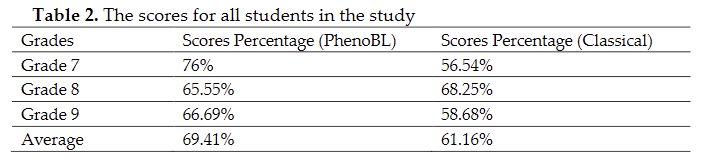
\includegraphics [width=0.9\textwidth] {table.png}

Ako ukazuje tabulka, úspešnosť je v priemero o 8\% vyššia pri vzdelávaní na základe fenoménov ako pri tradičnom vzdelávaní, avšak v 
ôsmej triede je úspešnosť vyššia pri tradičnom vzdelávaní. Toto môže byť zapríčinené či už veľmi malou vzorkov študentov alebo je
tradičné vzdelávanie pri velmi dobrom pomere žiakov k učitelom lepšie, pretože sa tam nájde viac priestoru pre zapájanie sa študentov,
čo tradičné vzdelávanie velmi vylepší. Takýto scenár je ajtak veľmi nereálny keďže možnosť vyrtvárať takto extrémne malé triedy môže byť iba
na súkromných školách.

Neskôr po teste študenti vypĺnali dotazník kde mali uviesť či by vedeli použiť znalosti a zručnosťi ktoré nadobudly počas štúdia. Približne 53\%
študentov odpovedalo že by ich dokázali použiť. To indikuje že použitie vzdelávania na základe fenoménov pomáha študentom použiť nadobudnuté 
znalosti a zručnosti omnoho dlhšie.

\subsection{Indonézia}

Štúdia z indonézie \cite{Santhalia_2020} sa zaoberala budovaním zručnosti na riešenie problémov v téme teplota a rozpínanie vdaka vzdelávaniu pomocou fenoménov.
Pri tomto výskume sa použila zmes rôznych metód s návrhom výskumu vloženého experimentálneho modelu. Do výskumu bolo zapojených tridsaťdva študentov
jedenásteho ročníka vyššej štátnej strednej školy v Malangu vo východnej Jave v Indonézií. Pred a po štúdiu dostali študenti test na otestovanie zručnosti riešenia problémov.

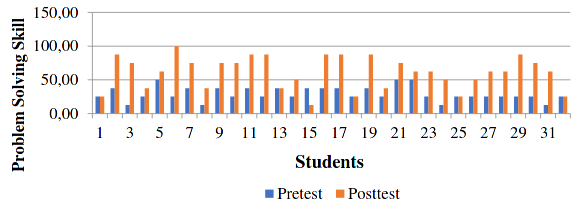
\includegraphics [width=0.9\textwidth] {graph.png}

Na grafe môžeme vidieť že väčšine študentov sa zručnosti riešenia problémov zlepšili po vzdelávaní pomocou fenoménov. Okolo 62,5\% študentov sa zručnosti riešenia problémov zlepšili.
Dáta ukazujú že keď študenti dostanú špecifický problém, tak vedia identifikovať jednotlivé zložky daného problému a vedia vytvoriť schému na jeho riešenie.


\section{Záver}

Výsledký o vzdelávaniana základe fenoménov nachádzajú zlepšenie vo výsledkoch študentov. Fínsko po implementácii
tohoto vzdelávacieho systému priamo do školstva v celej krajine sa stále drží medzi top krajinami na svete a zaznamenalo 
nárast úspešnosti študentov. Systém sa javý ako veľkým zlepšením oproti predchádzajúcemu avšak úpravu budú potrebujú aj
štandardizované testy ktoré su priamo viazané na naspameť fakty na ktoré nieje kladený z dobrých dôvodov dôraz.
\cite{pblf}

\bibliography{literature}
\bibliographystyle{unsrt}

\end{document}